\documentclass{article}

\usepackage{amsfonts,amsmath,amssymb}
\usepackage{hyperref}
\usepackage{graphicx}

\author{Ali Dorostkar \and Anastasia Kruchinina}
\title{\textsc{A new teaching style in computer programming}}
\date{\today}

\begin{document}

\maketitle \begin{abstract}
In this project we introduce a teaching technique for fields that require
practical work in order to be understood deeply. The focus of this article is 
to provide ways to simulate deep learning among students. To this end we describe 
details of a lecture session tailored specifically for Programming courses
where the students learn by participating, participating and other methods.
\end{abstract}

\section{Introduction} % (fold)
\label{sec:introduction}

Nowadays computers become an essential part of our lives.  \emph{``I have always wished
for my computer to be as easy to use as my telephone; my wish has come true
because I can no longer figure out how to use my telephone.'' - Bjarne
Stroustrup.}  

Programming is among the first courses that computer science students take.
There is a variety of programming languages which are thought in introductory
courses to programming ~\cite{de2002language}. Over the past years teachers
discussed on ways of teaching and the contents of a programming courses.

The outline of the report is as follows; In Section~\ref{sec:plan} we present the expected learning outcome of the course and define structure of the new lecture. We present the tools and facilities needed in order to be able to give this lecture. In Section~\ref{sec:analysis} the lecture is analysed, the possible implications of this model on student learning is predicted and we also show that such lecture would fulfil the requirements of the course. Finally we conclude the report in Section~\ref{sec:conclusion} where we give general comments and future plan for the presented model.

\section{What does it mean to teach programming?}


\emph{``For a long time it puzzled me how something so expensive, so leading edge,
could be so useless. And then it occurred to me that a computer is a stupid
machine with the ability to do incredibly smart things, while computer
programmers are smart people with the ability to do incredibly stupid things.
They are, in short, a perfect match. - Bill Bryson''.}

In our opinion, to program means to interact with computers, explain your will
to the machine and watch it execute your commands to the later. To teach
programming to students means to describe to them this interaction between human
and computer, express the language that one communicates with this stupid
machine, explain what the students should expect when they run a program and how
the students should deal with different ``surprises'' which computer may
produce, in particular how to debug the code efficiently.

In~\cite{state_of_art} the authors separate a process of writing the program
into two phases. The problem solving phase includes understanding the task
and designing the algorithm to reach the solution. This phase requires the
knowledge of the computer science concepts, software design techniques, critical
thinking skills and ability to think abstractly. In the second phase, called
implementation phase, the ideas obtained in the problem solving phase are
expressed in the executable form, translated into a programming language.

To master the implementation phase student must learn syntax of a chosen
programming language and be familiar with the development environment. It is
common that novice students struggle to learn the most basic programming
constructs, such as conditional and loop statements. This is due to the fact
that the implementation is reliant on problem solving and that by merely
teaching the syntax of a language, we are not providing enough information to
trigger deep learning, or as \emph{Eric S. Raymond} puts it 
\emph{``Computer science education cannot make anybody an expert programmer any
more than studying brushes and pigment can make somebody an expert painter''}. 

\section{Teaching methods}

The traditional approach in teaching programming courses includes lectures and
laboratory sessions. During the traditional lecture the teacher covers the
main concepts and shows examples, while students are in general passive
recipients of the information. During the lab sessions students solve practical
assignments and examine individually the results. It is common that large groups
of students are involved in the programming classes. Thus students usually work
in small groups (2-3 persons) during the lab sessions. 

According to Wirth~\cite{wirth}, the traditional lecturing has a number of
limitations.  ``Firstly, students' attention to what the instructor is saying
(i.e. their ability to concentrate) decreases as the lecture proceeds. This lack
of attention manifests itself in a reduction in the amount of information
retained by the student. For the first 5-10 minutes of a typical 50-minute
lecture a student remembers a high proportion of the information presented,
after which the proportion of information preserved rapidly declines. Students
typically retain 70\% from the first 10 minutes of lecture, and 20\% from the
last 10 minutes.''

Moreover, the amount of the information stored in the long-term memory depends
on the method of presenting informations, in particular in the amount of
interaction with students.  Studies show that just 10\% of information  is
retained in the long-term memory when person is reading, 50\% when hearing and
seeing, 90\% when doing and discussing, and 95\% when teaching and
tutoring~\cite{magnesen}. Therefore, one can conclude that the traditional
lecturing techniques does not suit teaching of the programming courses.
\emph{``In theory, theory and practice are the same. In practice,
they’re not. - Yoggi Berra'' }



A good overview of the existing programming teaching methods is given
in~\cite{mohorovivcic2011overview}. Authors pointed out the importance
of the deep learning: ``In programming, surface learning can be used
for memorising the language’s syntax, but deep learning is crucial, in
addition to surface learning, for gaining a true understanding of
programming logic and consequently a true competence in
programming''.

The problem-based learning might be a good alternative to the
traditional lecturing.  The problem introduced to the students should
be centered around the real practical problems. Students then discuss
the problem in groups and identify what they need to solve the
problem, what do they know and what should be learned. Then the
teacher present leanguage concepts and elements in the order the
students need to solve the problem. Every time students build
on their work from the week before. This lets students build a
substantial application that does real work.


The lab sessions may be organized in different ways. Students are
provided with a number of tasks to solve. As interesting task could
suggested by a puzzle-based
learning~\cite{mohorovivcic2011overview}. The problem is introduced to
students and then the code is separated into the very small parts
(puzzle pieces). Students must reconstruct the program by putting
parts in the correct order. To procedure can be automated or guided by
a teacher. Another example of the lab task could be to ask students to
provide an example of a program which uses just learned programming
concept.


The teacher may demonstrate to the students a badly written program which does
not behave correctly. The goal of such examples is to teach students
the good practices and get them excited about the development
of skills allowing to write good code.



\section{Practical experiences}


In programming courses students usually have different backgrounds,
various learning habits and motivation to study. As
pointed out in~\cite{experiment_iceland_2006} ``some of the students
have better preparation than the others and want to start programming
right away and are not willing to follow the teacher's instructions or
wait for other students. They want to work on their on own pace and
want the teacher to come running to help them when they are stuck.''.
The paper describes an experiment which was performed in the Reykjavik
University. The idea was to remove completely traditional lecture and
instead do more lab sessions (workshops). ``The teachers might give
short presentations, 5 – 10 minutes, at the beginning of the workshop,
or in between, that could be recorded, but mainly the students were
working on their tasks\ldots. When they see they need more knowledge
or help they are able to look through the recorded material and listen to the
teacher and do not have to wait for him. \ldots Students solve
exercises at very different speed and if they can find help in the
recorded material to keep on working they do not have to wait for the
teacher. The teacher can spend more time on students that need more
help than the recorded lectures can give them or want some extra
explanations; i.e. the teacher has more time for those who ask for
help and really need it.'' The overall experience was positive for
both students and teachers.

Similar experience is described in~\cite{cordes2002active}, where a
typical class consists of a series of mini-lectures and team-based
activities.  In addition, authors provide a concrete example of the
lecture structure discussing while-loops. The conclusion was that
``students are more engaged in this environment, and appreciate the
ability to interact with their classmates and instructor.''.

In the course ``Programming of Parallel Computers'' given by Uppsala university, 
the teachers implemented flipped classroom teaching method where the
lectures are available online\footnote{\url{www.scalablelearning.com}}
and the lectures' time are spent looking through different examples
where the students try to solve short programming problems. After each
exercise the teacher shows his solution and discusses the code. We
analyzed the course evaluation and for reduced the answers to above
and below average score. We see that of all students in the course
\begin{itemize}
	\item $62\%$ of the attendees think that the course quality is
		above average while $38\%$ are disappointed with the
		overall quality.
	\item $92\%$ of the students think that the course difficulty
		was above average.
	\item $100\%$ think that the amount of work was appropriate
		with regards to the attained credits.
	\item Everyone thought that the course is relevant for them.
	\item $84\%$ believed that the course is interesting while the
		remaining $16\%$ didn't agree.
	\item $74\%$ believed that their prior knowledge has helped
		them in understanding the course.
	\item Half the class expressed (using text comments in the
		positive opinion section) that the flipped classroom has helped them.
	\item In the negative opinions section, the students demanded
		a broader use of flipped classroom in the course.
	\item More than $60\%$ of the class thought that the
		traditional lecture hasn't helped them.
	\item $88\%$ thought that the flipped classroom has
		contributed to their learning.
	\item All students agreed that the labs and assignments were helpful in
		understanding the content.
	\item Almost $90\%$ didn't answer or should negative opinion
		regarding the helpfulness of the books and notes.
\end{itemize}
From the above points we can deduce that the students in this
programming course prefer hands-on approach, meaning that, they have
learned better by performing the task instead of sitting in the class
passively. We also see that although the students' opinion are
positive towards flipped classrooms, there is still space for
improvement since almost $40\%$ of the class think that the course
quality could be better and $70\%$ have relied on their prior
knowledge to get through the course.

As a complementary analysis of the flipped classroom and hands-on
technique, the teachers introduced each model separately and looked at
the final grades of the students. Figure~\ref{fig:grades} shows the
results of this study. We can clearly see the positive effect of the
flipped classroom and hands-on sessions. The students' grades are
generally shifted to the right (i.e higher grades).

\begin{figure}[htbp]
	\centering
	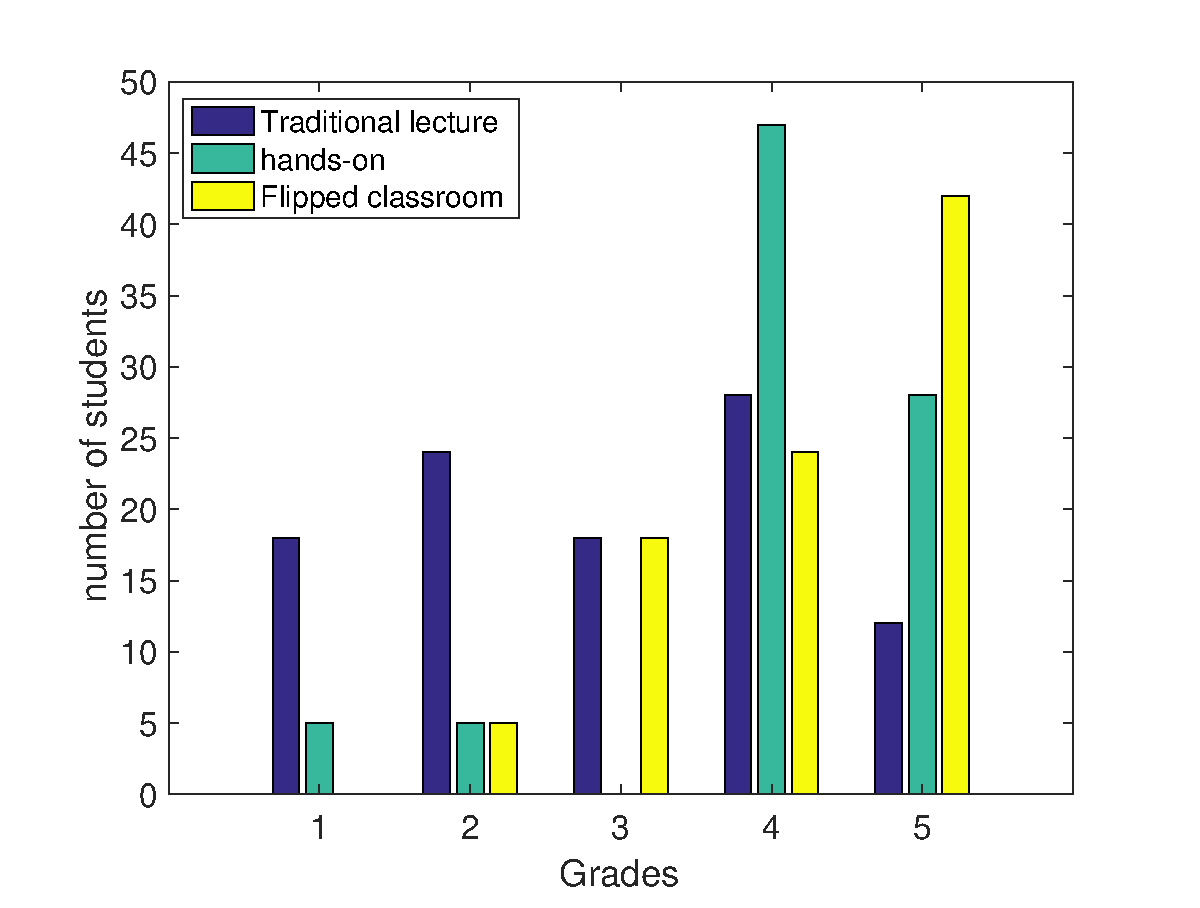
\includegraphics[width=0.95\textwidth]{fliped_effect.eps}
	\caption{The effect of flipped classroom on the grades of students}
	\label{fig:grades}
\end{figure}


In another attempt to reduce the gap between ``theory'' and ``practice'', the authors have tried a session where the Lab exercise and its corresponding lecture was mixed. In this lecture format, the teachers would teach part of the lecture and ask the students to work with it and implement a program. The overall student experience was positive but there were a few issues regarding the format. First, the size of the tasks and the amount of time for each ``mini-lecture'' should be tweaked. Next, the level of difficulty of each task needs to be taken into account and finally, the ultimate goal of the each lecture is better to be connected to real life applications either in the field of the students or from some common experience.


%(!!!COMMENT!!! I think the intro is complete. We have to correct the text later.)
%(!!!COMMENT!!! this part is the guideline for us, this will not be included in the final report.)
%\begin{itemize}
%	\item Write list of needs for a programming class
%	\item Present the required learning outcomes of a programming
%          course (The book of Biggs might be helpfull, added to git)
%	\item Define the structure of this lecture type
%	\item Study and predict the possible outcomes of the lecture
%	\item Describe how the lecture stimulates deep learning.
%	\item Present the tools that the teacher may use in the lecture.
%\end{itemize}
%% section introduction (end)
%
%\section{Approach} % (fold)
%\label{sec:plan}
%
%\url{http://www.socrative.com}\\
%\url{https://www.scalable-learning.com/}\\ %this is an in-house website from UU
%\url{https://getkahoot.com}\\
%\url{https://plickers.com}
%
%% section plan (end)
%\section{Analysis} % (fold)
%\label{sec:analysis}
%=======


%(!!! COMMENT: I don't think Ali's experience is needed, what Jarmo
%gave us is with evidence )
%(!!! COMMENT: I think here is a good example of a sample lab-lecture, I think
%similar as Ali did )




\section{Levels of thinking about the teaching}


The teacher's attitude to the teaching is very important. If teacher is not motivated or does not expect students willing to learn, no teaching methods will help to improve. Biggs~\cite{biggs2011teaching} presents three levels of thinking about
the teaching.  Jenkins~\cite{journey_Jenkins} discusses these levels,
and pointing out that every teacher moving through these levels as
they gain more experience. The first level includes transmitting
information, the responsibility for learning is lying totally on
students. The second level still includes elements of information
transmission, but more focusing on deep learning and activities where
students actively participate.  The third, and the best level, is
focusing just on the activities engaging students to learn. Teaching
is a process of motivation, the goal is ``to persuade the students
that learning to program (and so programming) is a good thing''. It is
pointed out in~\cite{journey_Jenkins} that in order to learn
something, students must be motivated and they ``must expect to
succeed''. Thus the role of the teacher is to provide students with framework and tools  they need to master a subject, interact with students and provide all needed information.





%say something about why.
%same something about what you have done in high performance, mixing lab lecture,
%also talk about the issues you had in this lab lecture
%\begin{itemize}
%	\item Write list of needs for a programming class
%	\item Present the required learning outcomes of a programming
%          course (The book of Biggs might be helpfull, added to git)
%	\item Define the structure of this lecture type
%	\item Study and predict the possible outcomes of the lecture
%	\item Describe how the lecture stimulates deep learning.
%	\item Present the tools that the teacher may use in the lecture.
%\end{itemize}
%% section introduction (end)
%
%\section{Approach} % (fold)
%\label{sec:plan}
%
%\url{http://www.socrative.com}\\
%\url{https://www.scalable-learning.com/}\\ %this is an in-house website from UU
%\url{https://getkahoot.com}\\
%\url{https://plickers.com}
%
%% section plan (end)
%\section{Analysis} % (fold)
%\label{sec:analysis}



%\vskip 10 pt
%See also, maybe good
%http://dl.acm.org/citation.cfm?id=2662412
%\vskip 10 pt




% section analysis (end)

\section{Conclusion} % (fold)
\label{sec:conclusion}


In this report we provide a brief review of the literature on the various teaching methods used in programming courses. 
We analyze a course evaluation of the programming course at Uppsala university and evaluate traditional lecturing, flipped classroom and hands-on approaches. The main conclusion drawn from the practical experiences is that the active learning facilitates deep learning and students in general prefer doing and discussing the material instead of passively listening to the teacher.

\bibliography{biblio} \bibliographystyle{siam} % achemso, apsrev


% section conclusion (end)
\end{document}
